\documentclass[11pt,a4paper]{article}

\usepackage[T1]{fontenc}
\usepackage[utf8]{inputenc}
\usepackage{amsmath}
\usepackage{microtype}
\usepackage[margin=1in]{geometry}
\usepackage{array,booktabs,tabularx}
\usepackage[dvipsnames]{xcolor}
\usepackage{tikz}
\usetikzlibrary{positioning,arrows.meta,calc,decorations.pathreplacing}
\usepackage{listings}
\usepackage[font=small,labelfont=bf]{caption}
\usepackage{enumitem}
\usepackage[colorlinks,linkcolor=MidnightBlue,urlcolor=MidnightBlue]{hyperref}
\usepackage[nameinlink]{cleveref}

\newcommand{\lang}{Boot}
\newcommand{\ext}{\texttt{.bt}}

\newcommand{\kw}[1]{\textbf{\texttt{#1}}}
\newcommand{\nt}[1]{\textit{#1}}
\newcommand{\tok}[1]{\texttt{"#1"}}
\newcommand{\hx}[1]{\texttt{0x#1}}
\newcommand{\vm}{VM16}
\newcommand{\op}[1]{\texttt{#1}}

\definecolor{codec}{HTML}{FCE8D2}
\definecolor{heapc}{HTML}{DDF0DC}
\definecolor{stackc}{HTML}{DCE9F7}

\lstdefinelanguage{boot}{morekeywords={fn,var,if,else,while,for,in,return,break,continue,nil,true,false},
  sensitive=true, morecomment=[l]{//}, morestring=[b]", morestring=[b]'}
\lstset{language=boot, basicstyle=\ttfamily\small, keywordstyle=\bfseries,
  commentstyle=\color{black!55}, columns=fullflexible, keepspaces,
  frame=single, rulecolor=\color{black!30}, xleftmargin=6pt, xrightmargin=6pt,
  aboveskip=8pt, belowskip=8pt}
\lstdefinestyle{shell}{language={}, keywordstyle={}, frame=none, backgroundcolor=\color{black!4}}

\tikzset{>=Stealth, every picture/.append style={font=\small}}
\setlength{\parskip}{3pt}

\title{\lang: a Small Self-Hosting Language for \vm{}\\[4pt]
\large Specification, version 0.1 (draft)}
\author{}
\date{\today}

\begin{document}
\maketitle

\begin{abstract}
\noindent
\lang{} is a small imperative language with dynamic types, C-style braces,
and one data structure: the dictionary. It is designed for one purpose: to
compile itself on \vm{}, running on a real Z80 or 6502 with 64\,KB of
memory. This document defines its syntax (in BNF), its values and their
meaning, the representation of values and programs on \vm{}, and the plan for
bootstrapping the compiler.
\end{abstract}

% =====================================================================
\section{Goals}

\begin{enumerate}[nosep]
\item \textbf{Self-hosting on 8-bit hardware.} The compiler is written in
  \lang{}, and it compiles itself on \vm{} within 64\,KB. Every decision
  below is measured against this.
\item \textbf{Simple to compile.} A one-pass recursive-descent compiler,
  with no syntax tree, emits \vm{} code directly, in the tradition of PL/0,
  Small-C and BCPL.
\item \textbf{Pleasant enough to write a compiler in.} Strings, dictionaries,
  recursion and character I/O; no type declarations.
\end{enumerate}
Non-goals: speed, floating point, closures, a large library, and integers
wider than 15 bits.

% =====================================================================
\section{A first example}

\begin{lstlisting}
// Count the words on standard input, and print each with its count.
var counts = {};

fn word() {                     // the next word, or nil at end of input
    var c = getc();
    while (c == ' ' || c == '\n') { c = getc(); }
    if (c < 0) { return nil; }
    var buf = [];               // a dictionary with keys 0, 1, 2, ...
    while (c >= 0 && c != ' ' && c != '\n') {
        buf[len(buf)] = c;
        c = getc();
    }
    return str(buf);
}

fn main() {
    var w = word();
    while (w != nil) {
        if (counts[w] == nil) { counts[w] = 0; }
        counts[w] = counts[w] + 1;
        w = word();
    }
    for (w in counts) { print(w); putc(' '); print(counts[w]); putc('\n'); }
}
\end{lstlisting}

A program is a series of global variable and function definitions. Running
it initialises the globals in order and then calls \texttt{main()}.

% =====================================================================
\section{Lexical structure}

\begin{center}
\small
\begin{tabularx}{\linewidth}{@{}l X@{}}
\toprule
token & form\\
\midrule
name & a letter or \texttt{\_}, then letters, digits and \texttt{\_}\\
integer & decimal digits, or \texttt{0x} and hexadecimal digits; at most \hx{7FFF}, taken modulo $2^{15}$\\
character & \texttt{'a'}: one character or escape between single quotes; its value is an integer\\
string & \texttt{"text"}: characters and escapes between double quotes\\
escape & \texttt{\textbackslash n \textbackslash t \textbackslash r \textbackslash 0 \textbackslash\textbackslash{} \textbackslash' \textbackslash\textquotedbl{} \textbackslash x}$hh$\\
keyword & \kw{fn var if else while for in return break continue nil true false}\\
operator & \texttt{( ) \{ \} [ ] , ; : .\ = == != < <= > >= + - * / \% ! \&\& ||}\\
comment & \texttt{//} to the end of the line\\
\bottomrule
\end{tabularx}
\end{center}
Spaces, tabs and newlines separate tokens and have no other meaning. Names
are case-sensitive.

% =====================================================================
\section{Grammar}

In the grammar, $\{\,x\,\}$ means zero or more $x$, $[\,x\,]$ means an
optional $x$, and quoted text is a token. Precedence is encoded in the
grammar, loosest first; all binary operators are left-associative except the
comparisons, which do not associate (\verb|a < b < c| is an error). The
whole grammar is in \cref{fig:grammar}.

\begin{figure}[t]
\centering
\renewcommand{\arraystretch}{1.15}
\begin{tabular}{@{}r@{\quad}c@{\quad}l@{}}
\nt{program}  & ::= & $\{$ \nt{global} $\}$\\
\nt{global}   & ::= & \nt{vardecl} $\mid$ \nt{fndef}\\
\nt{fndef}    & ::= & \tok{fn} \textsc{name} \tok{(} [ \nt{params} ] \tok{)} \nt{block}\\
\nt{params}   & ::= & \textsc{name} $\{$ \tok{,} \textsc{name} $\}$\\
\nt{vardecl}  & ::= & \tok{var} \textsc{name} [ \tok{=} \nt{expr} ] \tok{;}\\[5pt]
\nt{block}    & ::= & \tok{\{} $\{$ \nt{stmt} $\}$ \tok{\}}\\
\nt{stmt}     & ::= & \nt{vardecl} $\mid$ \nt{block} $\mid$ \nt{if}\\
              & $\mid$ & \tok{while} \tok{(} \nt{expr} \tok{)} \nt{block}\\
              & $\mid$ & \tok{for} \tok{(} \textsc{name} \tok{in} \nt{expr} \tok{)} \nt{block}\\
              & $\mid$ & \tok{return} [ \nt{expr} ] \tok{;}
                $\;\mid\;$ \tok{break} \tok{;} $\;\mid\;$ \tok{continue} \tok{;}\\
              & $\mid$ & \nt{expr} [ \tok{=} \nt{expr} ] \tok{;}\\
\nt{if}       & ::= & \tok{if} \tok{(} \nt{expr} \tok{)} \nt{block} [ \tok{else} ( \nt{block} $\mid$ \nt{if} ) ]\\[5pt]
\nt{expr}     & ::= & \nt{and} $\{$ \tok{||} \nt{and} $\}$\\
\nt{and}      & ::= & \nt{compare} $\{$ \tok{\&\&} \nt{compare} $\}$\\
\nt{compare}  & ::= & \nt{sum} [ ( \tok{==} $\mid$ \tok{!=} $\mid$ \tok{<} $\mid$ \tok{<=} $\mid$ \tok{>} $\mid$ \tok{>=} ) \nt{sum} ]\\
\nt{sum}      & ::= & \nt{product} $\{$ ( \tok{+} $\mid$ \tok{-} ) \nt{product} $\}$\\
\nt{product}  & ::= & \nt{unary} $\{$ ( \tok{*} $\mid$ \tok{/} $\mid$ \tok{\%} ) \nt{unary} $\}$\\
\nt{unary}    & ::= & ( \tok{-} $\mid$ \tok{!} ) \nt{unary} $\mid$ \nt{postfix}\\
\nt{postfix}  & ::= & \nt{primary} $\{$ \tok{(} [ \nt{args} ] \tok{)} $\mid$ \tok{[} \nt{expr} \tok{]} $\mid$ \tok{.} \textsc{name} $\}$\\
\nt{args}     & ::= & \nt{expr} $\{$ \tok{,} \nt{expr} $\}$\\
\nt{primary}  & ::= & \textsc{name} $\mid$ \textsc{integer} $\mid$ \textsc{character} $\mid$ \textsc{string}
                $\mid$ \tok{nil} $\mid$ \tok{true} $\mid$ \tok{false}\\
              & $\mid$ & \tok{(} \nt{expr} \tok{)} $\mid$ \nt{dict} $\mid$ \nt{list}\\
\nt{dict}     & ::= & \tok{\{} [ \nt{entry} $\{$ \tok{,} \nt{entry} $\}$ ] \tok{\}}\\
\nt{entry}    & ::= & ( \textsc{name} $\mid$ \textsc{string} $\mid$ \textsc{integer} $\mid$ \textsc{character} ) \tok{:} \nt{expr}\\
\nt{list}     & ::= & \tok{[} [ \nt{args} ] \tok{]}\\
\end{tabular}
\caption{The grammar of \lang.}
\label{fig:grammar}
\end{figure}

\paragraph{Notes.}
\begin{itemize}[nosep]
\item Braces are required around every body, so there is no dangling
  \kw{else}. A \nt{block} as a statement and a \nt{dict} as an expression
  never meet: a statement cannot start with \tok{\{} as an expression.
\item In \nt{expr} \tok{=} \nt{expr}, the left side must be a
  \textsc{name}, or a \nt{postfix} ending in \tok{[}\ldots\tok{]} or
  \tok{.}\textsc{name}. Assignment is a statement, not an expression.
\item The grammar is LL(1): one token of lookahead decides every choice.
  Whether an expression statement is an assignment is only known at the
  \tok{=}; the compiler keeps the code for the last indexing step pending
  until then (\cref{sec:compiler}).
\end{itemize}

% =====================================================================
\section{Values and meaning}\label{sec:values}

Every value has one of five types:

\begin{center}
\small
\begin{tabularx}{\linewidth}{@{}l X@{}}
\toprule
type & values\\
\midrule
nil & the single value \kw{nil}: the value of a missing key and of an
  uninitialised variable\\
integer & $-16384$ to $16383$. Arithmetic wraps modulo $2^{15}$. \kw{true} and
  \kw{false} are the integers 1 and 0\\
string & an immutable sequence of bytes. Strings are \emph{interned}: two
  strings with the same bytes are the same object\\
dictionary & a mutable map from keys (integers and strings) to values other
  than \kw{nil}\\
function & a function defined with \kw{fn}\\
\bottomrule
\end{tabularx}
\end{center}

\paragraph{Truth.} \kw{nil} and 0 are false; every other value is true.
\verb|!|, \verb|&&|, \verb!||! and the comparisons return 1 or 0, and
\verb|&&| and \verb!||! evaluate their right operand only when needed.

\paragraph{Operators.}
\begin{itemize}[nosep]
\item \verb|+ - * / %| take integers; \verb|/| and \verb|%| truncate towards
  zero, as in C, and division by zero is an error. \verb|+| also
  concatenates two strings.
\item \verb|< <= > >=| compare two integers, or two strings in byte order.
\item \verb|==| and \verb|!=| take any two values. Integers are equal when
  their values are; strings are equal when their bytes are, which by
  interning is the same as being the same object; dictionaries and functions
  are equal only to themselves.
\end{itemize}
Any other combination of operand types is a run-time error.

\paragraph{Dictionaries.} \verb|d[k]| is the value stored under key
\verb|k|, or \kw{nil}. \verb|d[k] = v| stores it, and storing \kw{nil}
removes the key. \verb|d.name| is short for \verb|d["name"]|. A key must be
an integer or a string. \verb|{a: 1, "b c": 2, 7: 3}| creates a dictionary;
a \textsc{name} before \tok{:} is a string key. \verb|[x, y, z]| is short
for \verb|{0: x, 1: y, 2: z}|.

\paragraph{Iteration.} \verb|for (k in d) {...}| binds the local variable
\verb|k| to each key of \verb|d| in turn: first the integer keys $0, 1, 2,
\ldots$ up to the first missing one, in increasing order, then the remaining
keys in the order they were first inserted. The order is therefore the same
on every implementation and every run, which the bootstrap test
(\cref{sec:bootstrap}) depends on. Adding or removing keys of \verb|d|
inside the loop is an error, or undefined if the implementation does not
check it.

\paragraph{Strings.} \verb|s[i]| is the byte at position \verb|i| (from 0)
as an integer, or \kw{nil} outside the string. Strings cannot be changed.

\paragraph{Variables and scope.} A \kw{var} at the top level declares a
global; one inside a function declares a local, visible from its declaration
to the end of the enclosing block. Parameters are locals. A name that is not
a local refers to a global, which may be declared later in the program, so
functions can call each other in any order. Every global that is used must
be declared somewhere, and no name may be declared twice in the same scope.

\paragraph{Functions.} Functions are values: they can be stored in variables
and dictionaries and called through them, \verb|ops.add(x, y)|. They are
defined only at the top level, so there are no closures. Calling a value
that is not a function, or with the wrong number of arguments, is an error.
A function that ends without \kw{return} returns \kw{nil}. Arguments are
evaluated left to right.

\paragraph{Errors.} A run-time error prints a message and stops the program
with exit status 1. There is no way to catch an error.

% =====================================================================
\section{Built-in functions}

The built-ins are global functions with reserved names.

\begin{center}
\small
\begin{tabularx}{\linewidth}{@{}l X@{}}
\toprule
function & result\\
\midrule
\texttt{getc()} & the next byte of standard input, or $-1$ at end of input\\
\texttt{putc(c)} & writes the byte $c \bmod 256$\\
\texttt{putw(n)} & writes $n \bmod 2^{15}$ as a little-endian word, so that
  a compiler can write addresses up to \hx{7FFF}\\
\texttt{print(v)} & writes an integer in decimal, or a string's bytes\\
\texttt{len(v)} & the number of bytes of a string, or of keys of a dictionary\\
\texttt{str(d)} & the string whose bytes are \verb|d[0]|, \verb|d[1]|, \ldots{} up to the first missing key\\
\texttt{chr(c)} & the one-byte string with byte $c$\\
\texttt{type(v)} & \verb|"nil"|, \verb|"int"|, \verb|"str"|, \verb|"dict"| or \verb|"fn"|\\
\texttt{error(s)} & prints \verb|s| and stops with an error\\
\texttt{exit(n)} & stops with exit status \verb|n|\\
\bottomrule
\end{tabularx}
\end{center}

% =====================================================================
\section{Representation on \vm{}}\label{sec:repr}

This section is not part of the language; it is the plan for the first
implementation.

\paragraph{Values} are single 16-bit words, distinguished by their low bit
and their address:
\begin{center}
\small
\begin{tabular}{@{}l l@{}}
\toprule
word & value\\
\midrule
$2n+1$ (odd) & the integer $n$\\
0 & \kw{nil}\\
even, nonzero & the address of an object, whose first word gives its type\\
\bottomrule
\end{tabular}
\end{center}
Integer arithmetic on tagged words is cheap: $a+b$ is $a+b-1$, and a
comparison of two integers is a comparison of the words. This is the scheme
of the CAM and of the graph reducer in this repository.

\paragraph{Objects.} Every object starts with a header word holding its type
in the low 3 bits and a size above them. A \emph{string} holds its length,
a hash and its bytes. A \emph{dictionary} holds a count, an \emph{array part}
for the keys $0, 1, \ldots, n-1$ (one word per value), and a \emph{hash
part}: an array of entries (key, value) in insertion order, with an index of
small integers into it, as in CPython's compact dictionaries. The array part
is what makes a dictionary used as an array cost a word per element, and the
two parts together give the iteration order of \cref{sec:values}. A
\emph{function} holds its number of parameters, followed by its code.

\paragraph{Static objects.} String literals and functions are placed in the
code area by the compiler and are never freed. Objects outside the heap are
ignored by the collector, which therefore only needs to test whether a word
is an even address inside the heap.

\paragraph{Interning.} The runtime keeps a hash set of all strings. A
string is only created through it, so two equal strings are one object. The
set is weak: the collector removes strings that are not otherwise reachable.

\paragraph{Garbage collection.} Mark and sweep, not copying: a copying
collector would halve the usable heap. The roots are the data stack and the
global table. Free blocks are kept on a free list and joined during the
sweep.

\paragraph{Frames.} Arguments are pushed on the data stack left to right,
and \op{CALL} pushes the return address on the separate return stack, so the
data stack holds only values and saved frame pointers, which are never heap
addresses. The callee saves the frame pointer (a fixed register), pushes
\kw{nil} for each of its locals, and addresses parameters and locals as
\texttt{[fp$\pm$k]}. The result is returned in $r_0$.

\paragraph{Code.} The compiler generates code for a stack machine on
\vm{}'s data stack and calls runtime routines for everything that checks
types: arithmetic, comparison, indexing, calls through values. Compiled code
is larger and slower than it could be, but the compiler stays simple and the
runtime is shared.

\begin{figure}[t]
\centering
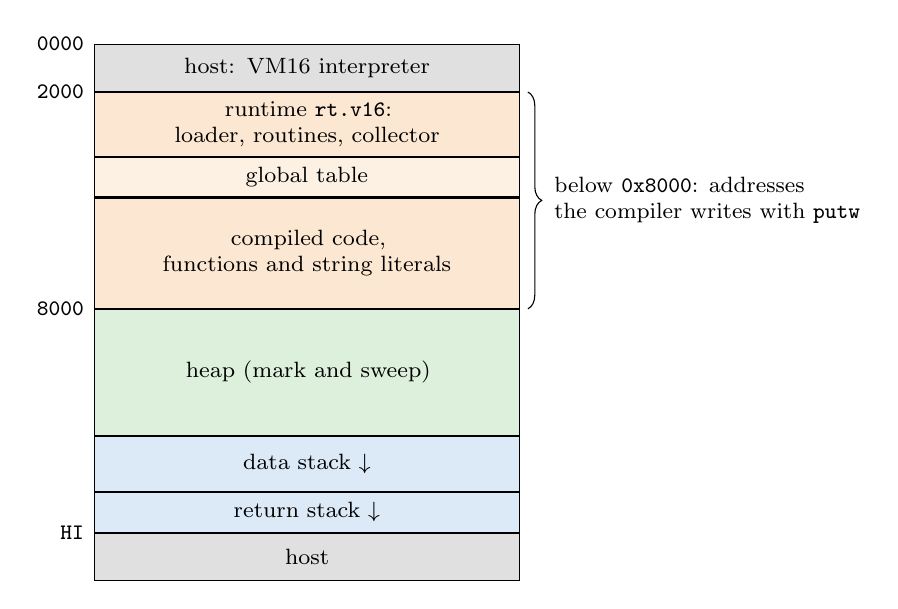
\begin{tikzpicture}[
  mem/.style={draw, text width=5.2cm, inner xsep=0.1cm, align=center, font=\footnotesize},
  adr/.style={font=\footnotesize\ttfamily, anchor=east}]
\node[mem, fill=black!12, minimum height=0.6cm] (m0) {host: \vm{} interpreter};
\node[mem, fill=codec, minimum height=0.8cm, below=0pt of m0] (m1) {runtime \texttt{rt.v16}:\\loader, routines, collector};
\node[mem, fill=codec!60, minimum height=0.5cm, below=0pt of m1] (m2) {global table};
\node[mem, fill=codec, minimum height=1.4cm, below=0pt of m2] (m3) {compiled code,\\functions and string literals};
\node[mem, fill=heapc, minimum height=1.6cm, below=0pt of m3] (m4) {heap (mark and sweep)};
\node[mem, fill=stackc, minimum height=0.7cm, below=0pt of m4] (m5) {data stack $\downarrow$};
\node[mem, fill=stackc, minimum height=0.5cm, below=0pt of m5] (m6) {return stack $\downarrow$};
\node[mem, fill=black!12, minimum height=0.6cm, below=0pt of m6] (m7) {host};
\node[adr] at (m0.north west) {0000};
\node[adr] at (m1.north west) {2000};
\node[adr] at (m4.north west) {8000};
\node[adr] at (m7.north west) {HI};
\draw[decorate, decoration={brace, amplitude=5pt}] ($(m1.north east)+(0.1,0)$) --
  node[right=6pt, align=left, font=\footnotesize] {below \hx{8000}: addresses\\the compiler writes with \texttt{putw}} ($(m3.south east)+(0.1,0)$);
\end{tikzpicture}
\caption{The planned memory map. \hx{2000} is where the Z80 build of \vm{}
loads images; HI is the top of the usable region from \texttt{SYS 2}.}
\label{fig:memory}
\end{figure}

% =====================================================================
\section{Programs and the compiler}\label{sec:compiler}

\paragraph{The object file.} A compiled program is not a \vm{} image. The
runtime \texttt{rt.v16} is the image: it reads the compiled program from the
start of standard input, places it in memory, and runs it; the rest of
standard input is the program's own input. This is how the graph reducer
reads its \texttt{.graph} files, and it means one fixed image on the target
machine, written in \vm{} assembly:
\begin{lstlisting}[style=shell]
cat prog.bto input.txt | vm16 rt.v16
\end{lstlisting}
An object file (\texttt{.bto}) is a sequence of chunks, each a kind byte, a
length word and that many bytes:
\begin{center}
\small
\begin{tabular}{@{}l l@{}}
\toprule
kind & meaning\\
\midrule
\texttt{C} & code: copied to the next free address of the code area\\
\texttt{S} & a string literal: copied, and entered in the intern set\\
\texttt{E} & the end; the body is the entry address, the initialisation code\\
\bottomrule
\end{tabular}
\end{center}
The compiler keeps the same running address as the loader, so it knows
where each chunk will land.

\paragraph{The compiler} reads the source once, with one token of lookahead,
and has no syntax tree: each parsing function emits code as it recognises
its construct.
\begin{itemize}[nosep]
\item The code for one function is collected in a dictionary of bytes
  (its array part), so that jumps within the function can be patched once
  their targets are known. At the end of the function it is written out as
  one \texttt{C} chunk and the dictionary is dropped. No more than one
  function's code is ever in memory.
\item An expression statement is compiled as an expression until the
  compiler sees whether \tok{=} follows. The last step of a \nt{postfix},
  \verb|[k]| or \verb|.name|, is therefore not emitted at once: the compiler
  emits the code for the dictionary and the key, and remembers that a
  \emph{get} is pending. If \tok{=} follows, it emits the value and a
  \emph{set} instead; otherwise it emits the \emph{get}. A plain
  \textsc{name} is handled the same way.
\item Globals are numbered in order of first use, and each has a slot in the
  global table. A call to a function, even one not yet defined, loads its
  global slot and calls through it, so no call ever needs patching.
\item Each string literal is written once, as an \texttt{S} chunk, the first
  time it is used. Because the loader interns these before the program
  runs, the literal is the string every later equal string will be.
\item The initialisers of the top-level \kw{var}s are collected as they are
  read, together with stores of each function into its slot, and written at
  the end, followed by a call to \texttt{main} and a halt. That is the
  \texttt{E} chunk.
\end{itemize}
At the end, the compiler reports any global that was used and never
declared.

% =====================================================================
\section{Bootstrapping}\label{sec:bootstrap}

\begin{enumerate}[nosep]
\item Write \texttt{rt.asm}, the runtime, in \vm{} assembly, and
  \texttt{btc.py}, a compiler from \lang{} to object files, in Python.
  \texttt{btc.py} is the reference, and is written in the style of \lang{}:
  one pass, no syntax tree, dictionaries only, so that it can be translated
  by hand almost line by line.
\item Write \texttt{btc.bt}, the same compiler in \lang{}, and test both on
  the same programs. Their output must be identical, byte for byte.
\item Compile \texttt{btc.bt} with \texttt{btc.py}, giving
  \texttt{btc1.bto}. Use it to compile \texttt{btc.bt} again:
\begin{lstlisting}[style=shell]
python3 btc.py btc.bt -o btc1.bto
cat btc1.bto btc.bt | vm16 rt.v16 > btc2.bto
cmp btc1.bto btc2.bto
\end{lstlisting}
  The two files must be identical: the compiler has reached a fixpoint.
\item Repeat the last step on the Z80 build of \vm{}. From then on
  \texttt{rt.v16} and \texttt{btc1.bto} are all the target needs.
\end{enumerate}

% =====================================================================
\section{Open questions}

\begin{itemize}[nosep]
\item \textbf{Will it fit?} The code area below \hx{8000} must hold the
  runtime, the global table and the compiled compiler; the heap above it the
  compiler's symbol table and one function's code. The first measurement
  should be the size of the compiled compiler and its peak heap use, under
  \texttt{btc.py} and \texttt{vm16 -c}, long before the Z80.
\item \textbf{15-bit integers.} Addresses from \hx{4000} to \hx{7FFF}
  appear as negative integers. Adding offsets to them works, because
  arithmetic wraps, but comparing them does not; the compiler should compare
  offsets, not addresses.
\item \textbf{Bit operations.} There are none: \verb|/| and \verb|%| are
  enough to split values into bytes. A compiler for an instruction set with
  bit fields would want \verb|&|, \verb.|. and shifts.
\item \textbf{Strings.} Is \texttt{str}, \texttt{chr} and \verb|+| enough
  string building? Each concatenation creates and interns a new string.
\item \textbf{Closures and nested functions} are left out on purpose; they
  would need environments on the heap.
\end{itemize}

\end{document}
